\chapter{Encodings}
\label{chap:encodings}

\section{Instruction Length and Alignment}
For this revision, PTO uses only 32-bit and 64-bit CPU-visible instruction units. Bit 0 is the least-significant bit of each 32-bit word. A 64-bit instruction is two adjacent 32-bit words shown in stream order, with the lowest-addressed word first. Encoders and disassemblers MUST preserve the decoded instruction boundary; exception reporting, speculation recovery, and retirement are attributed to the CPU-visible instruction or descriptor bundle, not to an internal expanded microcode site.

\begin{longtable}{@{}L{0.22\linewidth}L{0.20\linewidth}L{0.46\linewidth}@{}}
\toprule
Form & Length & Requirement \\
\midrule
Scalar/control instruction & 32 bits & Primary scalar/control form. Scalar register operands use 5-bit \texttt{X0}--\texttt{X31} fields. \\
Wide scalar/control instruction & 64 bits & Two 32-bit words decoded as one instruction. Used by profiles that need a full immediate, address, or metadata extension. \\
Tile/vector descriptor instruction & 32 or 64 bits & A descriptor instruction is either one 32-bit descriptor word or one 64-bit paired descriptor. Tile operations are represented as descriptor bundles made only from these 32-bit and 64-bit descriptor instructions. \\
Micro instruction & 64 bits & Fixed microcode word with \texttt{WM} in bits \texttt{31:0} and \texttt{WO} in bits \texttt{63:32}. It is UOP Engine state and is not fetched as a CPU instruction. \\
\bottomrule
\end{longtable}

A 64-bit instruction extension is part of the same decoded instruction as its first word. It extends opcode, immediate, or metadata fields; it does not define a second architectural operation. The authoritative meaning of every field is the instruction profile that names the opcode and format. This manual defines only the 32-bit and 64-bit forms.

\section{Scalar Instruction Encoding}
\label{sec:scalar_instruction_encoding}
The scalar ISA surface is encoded with opcode fields plus 5-bit scalar register fields. The register code \texttt{0b00000} names \texttt{X0}; \texttt{0b11111} names \texttt{X31}. This manual uses the field names below for scalar instruction diagrams and descriptor tables:

\begin{longtable}{@{}L{0.22\linewidth}L{0.18\linewidth}L{0.50\linewidth}@{}}
\toprule
Field & Width & Meaning \\
\midrule
\texttt{OPCODE} & profile-defined & Scalar or control operation selector. Reserved values are illegal. \\
\texttt{RegDst} & 5 & Destination scalar register \texttt{X0}--\texttt{X31}. Writes to \texttt{X0} are ignored. \\
\texttt{RegSrc0} & 5 & First scalar source register \texttt{X0}--\texttt{X31}. \\
\texttt{RegSrc1} & 5 & Second scalar source register \texttt{X0}--\texttt{X31}. \\
\texttt{RegSrc2} & 5 & Third scalar source register or scalar IO import \texttt{X0}--\texttt{X31}. \\
\texttt{IMM} & profile-defined & Immediate operand. Sign extension, zero extension, and scaling are defined by the opcode profile. \\
\bottomrule
\end{longtable}

The scalar encoding does not use tile bundled descriptors. Scalar arithmetic, branch, memory, and control forms keep their own opcode profiles and use scalar register fields directly. A scalar instruction is either a 32-bit instruction or a 64-bit wide instruction; the 64-bit form adds immediate or opcode space, not extra scalar architectural registers.

\section{Tile Instruction Encoding Formats}
\label{sec:tile_instruction_encoding_formats}
Tile instructions use a bundled descriptor format. A tile instruction begins with one required 32-bit \texttt{B.OP} header instruction and is followed by the \texttt{B.*} descriptors required by that tile opcode profile. Each descriptor word in this revision is 32 bits. The bundle is the CPU-visible tile operation unit: exception reporting and retirement are attributed to the whole descriptor bundle, not to each descriptor word independently.

Each per-instruction tile page specifies the exact ordered descriptor bundle for that catalog instruction and lists the concrete \texttt{B.OP.Opcode} value used by that instruction.

\begin{longtable}{@{}L{0.18\linewidth}L{0.18\linewidth}L{0.54\linewidth}@{}}
\toprule
Descriptor & Required & Role \\
\midrule
\texttt{B.OP} & yes & First tile descriptor carrying the opcode, data type, and profile selector. \\
\texttt{B.IOT}/\texttt{B.IOTI} & usually & Tile input/output binding with source lifecycle bits, source selectors, destination selector, and a profile-defined size field. The per-instruction tile catalog uses the immediate-size \texttt{B.IOTI} form unless a profile explicitly needs a scalar size source. \\
\texttt{B.IOR} & when scalar operands are imported & Scalar register binding using the common \texttt{X0}--\texttt{X31} encoding. \\
\texttt{B.DIM} & when explicit dimensions are needed & Shape, valid-region, or loop-bound descriptor. \\
\texttt{B.ARG} & profile-defined & Operation argument such as layout mode, scalar/tile operand mode, quantization mode, or transform selector. \\
\texttt{B.ATTR} & optional & Format override, layout override, mask mode, ordering, lifecycle, trap, or result-role attributes. \\
\texttt{B.TEXT} & only for out-of-line bodies & PC-relative body target. UOP Engine-generated tile operations do not use it. \\
\texttt{B.HINT} & optional & Performance hint. Hints do not change architectural state. \\
\bottomrule
\end{longtable}

\subsection{Descriptor Bundle Rules}
\begin{itemize}
\item \texttt{B.OP} MUST be the first descriptor in a tile instruction bundle.
\item The selected tile opcode profile defines the required descriptor sequence after \texttt{B.OP}. Extra descriptors and missing mandatory descriptors are illegal.
\item Descriptor order after \texttt{B.OP} is canonical: \texttt{B.ARG}, \texttt{B.ATTR}, \texttt{B.DIM}, \texttt{B.IOR}, tile IO descriptors (\texttt{B.IOT} or \texttt{B.IOTI}), \texttt{B.TEXT}, then \texttt{B.HINT}. Encoders SHOULD emit this order; decoders MAY reject non-canonical order.
\item Descriptors that are not required by the selected opcode MUST be absent unless the opcode profile explicitly accepts them.
\item If both \texttt{B.ATTR} and \texttt{B.OP} carry the same property, \texttt{B.ATTR} refines the \texttt{B.OP} default. The combination is illegal if the opcode profile does not define the refinement.
\item Register fields inside \texttt{B.IOR} use the scalar \texttt{X0}--\texttt{X31} encoding. Tile operand descriptors do not define \texttt{T}, \texttt{U}, or predicate register namespaces.
\end{itemize}

\subsection{\texttt{B.OP} --- Tile Operation Descriptor}
\label{sec:b_op}
\index{B.OP}\index{tile operation descriptor}

\texttt{B.OP} is the first descriptor in every PTO tile instruction bundle. It selects the tile instruction through an \texttt{Opcode} field and carries the element data type. The UOP Engine uses this descriptor together with the following descriptor words to generate the tile microcode body.

\begin{center}
\captionof{figure}{Bit allocation for the required \texttt{B.OP} descriptor word.}
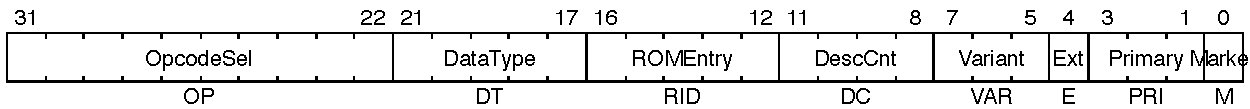
\includegraphics[width=0.95\linewidth]{figs/encoding/pto_b_op_instruction.pdf}
\end{center}

\begin{longtable}{@{}L{0.14\linewidth}L{0.20\linewidth}R{0.08\linewidth}L{0.48\linewidth}@{}}
\toprule
Bits & Field & Width & Meaning \\
\midrule
\texttt{31:27} & \texttt{DataType} & 5 & Element or accumulator data type selector. See Section~\ref{tab:format_sel}. \\
\texttt{26:25} & \texttt{Mode} & 2 & Tile descriptor mode. \\
\texttt{24:15} & \texttt{Opcode} & 10 & Tile opcode selector for the selected PTO tile instruction profile. \\
\texttt{14:12} & \texttt{Selector} & 3 & Fixed to \texttt{001}. \\
\texttt{11:7} & \texttt{Kind} & 5 & Tile descriptor kind. \\
\texttt{6:4} & \texttt{Major} & 3 & Fixed to \texttt{000}. \\
\texttt{3:1} & \texttt{Minor} & 3 & Fixed to \texttt{000}. \\
\texttt{0} & \texttt{Marker} & 1 & 32-bit instruction marker. Fixed to \texttt{1}. \\
\bottomrule
\end{longtable}

\subsection{Tile Operand Descriptors}
\label{sec:tile_operand_descriptors}
\texttt{B.IOT}/\texttt{B.IOTI} binds tile operands for the selected \texttt{B.OP}. Each descriptor carries up to two explicit source tile references and an arrow destination/size binding; repeated descriptors are consumed in header order when an opcode profile needs more tile inputs or additional binding groups. \texttt{B.IOTI} uses an immediate \texttt{SizeCode}. \texttt{B.IOT} is reserved for profiles that need the same source-list layout with a scalar size source register.

\begin{center}
\captionof{figure}{Bit allocation for the \texttt{B.IOTI} immediate-size tile operand descriptor used by generated PTO tile pages.}
\includegraphics[width=0.95\linewidth]{figs/encoding/pto_b_ioti_instruction.pdf}
\end{center}

\begin{longtable}{@{}L{0.20\linewidth}L{0.24\linewidth}L{0.46\linewidth}@{}}
\toprule
Field class & Descriptor fields & Meaning \\
\midrule
Lifecycle & \texttt{S0R}, \texttt{S1R}, absent bits & Source reuse or kill/default-release intent. \\
Source operands & \texttt{SrcTile0}, \texttt{SrcTile1} & Descriptor-local source tile operand selectors consumed by the tile opcode profile. \\
Destination & \texttt{DstTile} plus arrow suffix & Descriptor-local destination kind and allocation/size binding, printed as forms such as \texttt{->t<1KB>} or \texttt{->acc<4KB>}. \\
Size & \texttt{SizeCode/RegSrc} & Profile-defined tile size field. Immediate size codes are preferred; scalar register size sources are legal only when the opcode profile enables dynamic sizing. \\
Mask/predicate tile & opcode profile plus operand selector & A tile-shaped mask is encoded as an ordinary tile operand with a mask role declared by the tile opcode profile or \texttt{B.ATTR}. \\
\bottomrule
\end{longtable}

\subsection{Descriptor Profiles by Tile Family}
\label{sec:tile_descriptor_profiles}
Each tile instruction family defines a required descriptor profile. Missing mandatory descriptors and extra unsupported descriptors are illegal.

The reusable bit splits for \texttt{B.ATTR}, \texttt{B.DIM}, \texttt{B.IOR}, \texttt{B.IOT}/\texttt{B.IOTI}, and related descriptors are listed in Section~\ref{sec:bundled_descriptor_encoding}.

{\scriptsize
\begin{longtable}{@{}L{0.20\linewidth}L{0.36\linewidth}L{0.34\linewidth}@{}}
\toprule
Family & Required descriptors & Notes \\
\midrule
Tile-tile elementwise & \texttt{B.OP + B.IOTI} & \texttt{B.IOTI} binds up to two source tiles and the arrow destination. \\
Tile-scalar elementwise & \texttt{B.OP + B.ARG + B.IOR + B.IOTI} & \texttt{B.IOR} imports the scalar source. \texttt{B.IOTI} binds the source tile and arrow destination. \\
Unary and special math & \texttt{B.OP + B.ARG + B.IOTI} & Unused source fields are marked absent; the arrow suffix still binds the destination and size. \\
Axis reduce & \texttt{B.OP + B.ARG + B.DIM + B.IOTI} & \texttt{B.DIM} defines the reduction axis and valid bounds. \\
Axis expand and broadcast & \texttt{B.OP + B.ARG + B.DIM + B.IOTI} & \texttt{B.DIM} defines the expanded dimension and source valid range. \\
Partial and valid-region & \texttt{B.OP + B.ARG + B.ATTR + B.IOTI} & \texttt{B.ATTR} carries pad, mask, or valid-region behavior. \\
Select and predication & \texttt{B.OP + B.ARG + B.ATTR + B.IOTI...} & A tile-shaped mask is an ordinary tile input role; profiles with more than two tile inputs use repeated \texttt{B.IOTI} descriptors in header order. \\
Conversion & \texttt{B.OP + B.ARG + B.ATTR + B.IOTI} & \texttt{B.OP.DataType} selects the destination type; \texttt{B.ATTR} may carry source-format or rounding refinements. \\
\bottomrule
\end{longtable}
}

\section{Micro Instruction Encoding Formats}
\label{sec:micro_instruction_encoding}
Each static tile/vector micro instruction in a tile instruction body is encoded as one fixed 64-bit micro instruction. The low 32 bits are \texttt{WM}, the metadata half. The high 32 bits are \texttt{WO}, the operation half. The 64-bit word is UOP Engine state; the microassembler combines it with decoded \texttt{B.OP}, operand descriptors, dimension or attribute descriptors, and tile metadata to produce vector beat words.

The tables on each per-instruction tile page list the fixed 64-bit micro instruction sites for that microcode body. The \texttt{WO} and \texttt{WM} columns are the two encoded halves of the same 64-bit word, not separate instructions.

\begin{center}
\captionof{figure}{Bit allocation for one 64-bit PTO micro instruction. Bits \texttt{31:0} are \texttt{WM}; bits \texttt{63:32} are \texttt{WO}.}
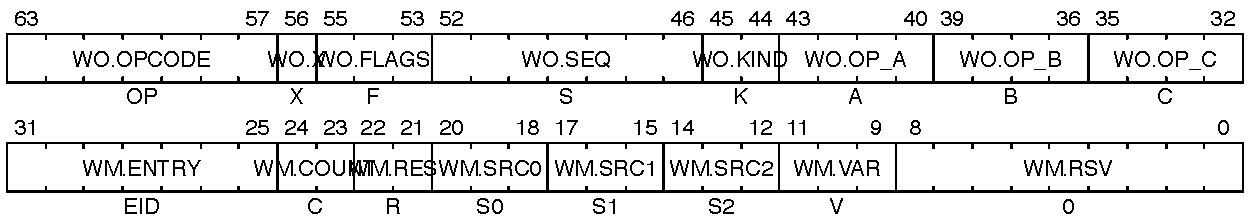
\includegraphics[width=0.95\linewidth]{figs/encoding/micro_64_instruction.pdf}
\end{center}

\begin{longtable}{@{}L{0.14\linewidth}L{0.20\linewidth}R{0.08\linewidth}L{0.48\linewidth}@{}}
\toprule
Bits & Field (attr) & Width & Meaning \\
\midrule
\multicolumn{4}{@{}l}{\textbf{WO: operation half, bits 63:32}} \\
\texttt{63:57} & \texttt{WO.OPCODE} (OP) & 7 & Micro instruction opcode. The current vector domain uses \texttt{u\_vec.*} mnemonics. See Section~\ref{sec:micro_instruction_opcode_map}. \\
\texttt{56} & \texttt{WO.IS\_EXT} (X) & 1 & Extension form bit for the micro instruction. Set to 1 when this micro instruction uses an extended operand encoding. \\
\texttt{55:53} & \texttt{WO.FLAGS} (F) & 3 & Operation class flags. Encodes the functional class of this micro instruction. Defined values are listed in Section~\ref{sec:wo_flags}. \\
\texttt{52:46} & \texttt{WO.SEQ} (S) & 7 & Static sequence number within the microcode body. Lower SEQ executes before higher SEQ. Two sites MUST NOT share the same SEQ value within one body. \\
\texttt{45:44} & \texttt{WO.OP\_KIND} (K) & 2 & Operand kind: 0 = unary, 1 = binary, 2 = ternary, 3 = control. \\
\texttt{43:40} & \texttt{WO.OP\_A} (A) & 4 & First operand slot selector for the expanded micro instruction. \\
\texttt{39:36} & \texttt{WO.OP\_B} (B) & 4 & Second operand slot selector. \\
\texttt{35:32} & \texttt{WO.OP\_C} (C) & 4 & Third operand or destination slot selector. \\
\midrule
\multicolumn{4}{@{}l}{\textbf{WM: metadata half, bits 31:0}} \\
\texttt{31:25} & \texttt{WM.ENTRY\_ID} (EID) & 7 & UOP Engine entry ID. Must match the entry selected by the decoded tile opcode profile for this tile instruction body. \\
\texttt{24:23} & \texttt{WM.OP\_COUNT} (C) & 2 & Number of operand slots used by this micro instruction site: 0 = control, 1 = unary, 2 = binary, 3 = ternary. \\
\texttt{22:21} & \texttt{WM.RES\_TYPE} (R) & 2 & Result class of this micro instruction. Defined values are listed in Section~\ref{sec:res_type}. \\
\texttt{20:18} & \texttt{WM.SRC0\_TYPE} (S0) & 3 & Type of the first source operand slot. Defined values are listed in Section~\ref{sec:src_type}. \\
\texttt{17:15} & \texttt{WM.SRC1\_TYPE} (S1) & 3 & Type of the second source operand slot. \\
\texttt{14:12} & \texttt{WM.SRC2\_TYPE} (S2) & 3 & Type of the third source operand slot. \\
\texttt{11:9} & \texttt{WM.VARIANT} (V) & 3 & Beat-word variant selector. Undefined variant values MUST be rejected by the microassembler. \\
\texttt{8:0} & \texttt{WM.RSV} & 9 & Reserved. Encoders MUST write zero. Decoders and microassemblers MUST ignore this field for this revision. \\
\bottomrule
\end{longtable}

\section{Encoding Field References}
\subsection{WO FLAGS Encoding}
\label{sec:wo_flags}
The WO FLAGS field (\texttt{F}) classifies each micro instruction site by its functional role. The flags determine routing in the micro instruction decoder and are validated against the opcode. Defined values are:

\begin{longtable}{@{}L{0.18\linewidth}L{0.14\linewidth}L{0.58\linewidth}@{}}
\toprule
Flag value (binary) & Flag name & Functional class \\
\midrule
\texttt{000} & \texttt{alu} & ALU arithmetic, logical, comparison, special-function, or data-format micro instruction. Routed to the vector ALU pipeline. \\
\texttt{001} & \texttt{mem} & Vector load or store micro instruction. Routed to the memory queue. \\
\texttt{010} & \texttt{setup} & Control or mask setup micro instruction. May initialize masks, broadcast scalars, or emit memory barriers. \\
\texttt{011} & \texttt{cmp} & Comparison micro instruction producing a mask result. Routed to the mask generation path. \\
\texttt{100} & \texttt{ctrl} & Control micro instruction, such as a branch, barrier, or other flow-modifying operation. \\
\texttt{101}--\texttt{111} & \texttt{reserved} & Reserved for this revision. \\
\bottomrule
\end{longtable}
\index{FLAGS}

\subsection{RES\_TYPE Encoding}
\label{sec:res_type}
The WM RES\_TYPE field (\texttt{R}) encodes the result class of the micro instruction:

\begin{longtable}{@{}L{0.18\linewidth}L{0.14\linewidth}L{0.58\linewidth}@{}}
\toprule
Value & Name & Result class \\
\midrule
\texttt{00} & \texttt{vec} & Vector result for the selected tile/vector payload. \\
\texttt{01} & \texttt{mask} & Mask result used for predicated operations. \\
\texttt{10} & \texttt{mem} & Memory side-effect result. The micro instruction performs a tile-payload or global-memory store. \\
\texttt{11} & \texttt{ctrl} & Control result, such as a barrier or control-flow micro operation. \\
\bottomrule
\end{longtable}
\index{RES_TYPE}

\subsection{SRC\_TYPE Encoding}
\label{sec:src_type}
The WM SRC\_TYPE fields (\texttt{S0}, \texttt{S1}, \texttt{S2}) encode the type of each source operand slot:

\begin{longtable}{@{}L{0.18\linewidth}L{0.18\linewidth}L{0.54\linewidth}@{}}
\toprule
Value & Name & Operand class \\
\midrule
\texttt{000} & \texttt{vec\_reg} & Vector payload operand selected by the decoded tile operand fields. \\
\texttt{001} & \texttt{vec\_imm} & Vector immediate operand, such as a broadcast scalar or inline constant. \\
\texttt{010} & \texttt{vec\_stg} & Vector staging operand, produced by a prior micro instruction within the same microcode body. \\
\texttt{011} & \texttt{mask\_reg} & Mask operand selected by decoded metadata. \\
\texttt{100} & \texttt{mask\_imm} & Immediate mask literal. \\
\texttt{101} & \texttt{idx\_reg} & Index operand, such as an address-calculation source. \\
\texttt{110} & \texttt{idx\_imm} & Immediate index operand. \\
\texttt{111} & \texttt{null} & No operand. Unary operations use this for unused source slots. \\
\bottomrule
\end{longtable}
\index{SRC_TYPE}

\subsection{FORMAT\_SEL Encoding}
\label{tab:format_sel}
The FORMAT\_SEL field (\texttt{FMT}) selects the element data type for the tile instruction. Defined values are:

\begin{longtable}{@{}L{0.18\linewidth}L{0.22\linewidth}L{0.50\linewidth}@{}}
\toprule
Value & Format name & Description \\
\midrule
\texttt{0x0} & \texttt{f16} & 16-bit IEEE 754 half-precision floating point. \\
\texttt{0x1} & \texttt{f32} & 32-bit IEEE 754 single-precision floating point. \\
\texttt{0x2} & \texttt{bf16} & 16-bit brain floating point (bfloat16). \\
\texttt{0x3} & \texttt{i8} & 8-bit signed integer. \\
\texttt{0x4} & \texttt{ui8} & 8-bit unsigned integer. \\
\texttt{0x5} & \texttt{si8} & 8-bit signed integer alias with profile-defined saturation or rounding behavior. \\
\texttt{0x6} & \texttt{i16} & 16-bit signed integer. \\
\texttt{0x7} & \texttt{ui16} & 16-bit unsigned integer. \\
\texttt{0x8} & \texttt{si16} & 16-bit signed integer alias with profile-defined saturation or rounding behavior. \\
\texttt{0x9} & \texttt{i32} & 32-bit signed integer. \\
\texttt{0xA} & \texttt{ui32} & 32-bit unsigned integer. \\
\texttt{0xB} & \texttt{si32} & 32-bit signed integer alias with profile-defined saturation or rounding behavior. \\
\texttt{0xC}--\texttt{0xF} & \texttt{reserved} & Reserved for this revision. \\
\bottomrule
\end{longtable}
\index{FORMAT_SEL}

\subsection{LAYOUT\_SEL Encoding}
\label{sec:layout_sel}
The LAYOUT\_SEL field (\texttt{LAY}) selects the memory layout interpretation of tile storage:

\begin{longtable}{@{}L{0.18\linewidth}L{0.22\linewidth}L{0.50\linewidth}@{}}
\toprule
Value & Layout name & Description \\
\midrule
\texttt{0x0} & \texttt{row\_major} & Elements stored in row-major order. Consecutive columns share the same row. \\
\texttt{0x1} & \texttt{col\_major} & Elements stored in column-major order. Consecutive rows share the same column. \\
\texttt{0x2}--\texttt{0xF} & \texttt{reserved} & Reserved for this revision. \\
\bottomrule
\end{longtable}
\index{LAYOUT_SEL}

\section{Tile Instruction Opcode Map}
This chapter lists all CPU-visible tile instruction entries and their microcode-site budgets in an aligned table. The opcode column is the tile catalog opcode used by this manual. \texttt{B.OP} carries the tile opcode; the selected tile opcode profile defines the following descriptors and maps the instruction to the UOP Engine entry.

\noindent\textbf{Extended opcode space (\texttt{0xF000}--\texttt{0xFFFF}).} Entries with opcodes in the \texttt{0xF000}--\texttt{0xFFFF} range are allocated from the extended opcode space reserved for specialized or infrequently used tile instructions. These opcodes are decoded with the domain field indicating the extended domain. Current entries in extended space: \texttt{0xF000} (trowargmax), \texttt{0xF001} (trowargmin), \texttt{0xF002} (trowexpanddiv), \texttt{0xF003} (trowexpandmul), \texttt{0xF004} (trowexpandsub), \texttt{0xF005} (trowprod).

{\scriptsize
\begin{longtable}{@{}R{0.045\linewidth}L{0.29\linewidth}L{0.12\linewidth}R{0.10\linewidth}R{0.10\linewidth}R{0.08\linewidth}@{}}
\toprule
ID & Tile instruction & Opcode & WO/WM sites & VEC sites & Bytes \\
\midrule
0 & \texttt{TABS} & \texttt{0x1006} & 3 & 3 & 24 \\
1 & \texttt{TADD} & \texttt{0x1007} & 4 & 4 & 32 \\
2 & \texttt{TADDS} & \texttt{0x1009} & 3 & 3 & 24 \\
3 & \texttt{TAND} & \texttt{0x100B} & 4 & 4 & 32 \\
4 & \texttt{TANDS} & \texttt{0x100C} & 4 & 4 & 32 \\
5 & \texttt{TCOLEXPAND} & \texttt{0x1010} & 2 & 2 & 16 \\
6 & \texttt{TCOLEXPANDADD} & \texttt{0x1011} & 4 & 4 & 32 \\
7 & \texttt{TCOLEXPANDDIV} & \texttt{0x1012} & 4 & 4 & 32 \\
8 & \texttt{TCOLEXPANDEXPDIF} & \texttt{0x1013} & 9 & 9 & 72 \\
9 & \texttt{TCOLEXPANDMAX} & \texttt{0x1014} & 4 & 4 & 32 \\
10 & \texttt{TCOLEXPANDMIN} & \texttt{0x1015} & 4 & 4 & 32 \\
11 & \texttt{TCOLEXPANDMUL} & \texttt{0x1016} & 4 & 4 & 32 \\
12 & \texttt{TCOLEXPANDSUB} & \texttt{0x1017} & 4 & 4 & 32 \\
13 & \texttt{TCOLMAX} & \texttt{0x1018} & 4 & 4 & 32 \\
14 & \texttt{TCOLMIN} & \texttt{0x1019} & 4 & 4 & 32 \\
15 & \texttt{TCOLPROD} & \texttt{0x101A} & 4 & 4 & 32 \\
16 & \texttt{TCOLSUM} & \texttt{0x101B} & 4 & 4 & 32 \\
17 & \texttt{TCVT} & \texttt{0x101C} & 15 & 15 & 120 \\
18 & \texttt{TDIV} & \texttt{0x101D} & 4 & 4 & 32 \\
19 & \texttt{TDIVS} & \texttt{0x101E} & 8 & 8 & 64 \\
20 & \texttt{TEXP} & \texttt{0x101F} & 3 & 3 & 24 \\
21 & \texttt{TEXPANDS} & \texttt{0x1020} & 2 & 2 & 16 \\
22 & \texttt{TFILLPAD} & \texttt{0x1023} & 8 & 8 & 64 \\
24 & \texttt{TLOG} & \texttt{0x1030} & 3 & 3 & 24 \\
25 & \texttt{TLRELU} & \texttt{0x1031} & 3 & 3 & 24 \\
26 & \texttt{TMAX} & \texttt{0x1034} & 4 & 4 & 32 \\
27 & \texttt{TMAXS} & \texttt{0x1035} & 3 & 3 & 24 \\
28 & \texttt{TMIN} & \texttt{0x1036} & 4 & 4 & 32 \\
29 & \texttt{TMINS} & \texttt{0x1037} & 3 & 3 & 24 \\
30 & \texttt{TMUL} & \texttt{0x103B} & 4 & 4 & 32 \\
31 & \texttt{TMULS} & \texttt{0x103C} & 3 & 3 & 24 \\
32 & \texttt{TNEG} & \texttt{0x103D} & 3 & 3 & 24 \\
33 & \texttt{TNOT} & \texttt{0x103E} & 3 & 3 & 24 \\
34 & \texttt{TOR} & \texttt{0x103F} & 4 & 4 & 32 \\
35 & \texttt{TORS} & \texttt{0x1040} & 4 & 4 & 32 \\
36 & \texttt{TPARTADD} & \texttt{0x1041} & 6 & 6 & 48 \\
37 & \texttt{TPARTMAX} & \texttt{0x1042} & 10 & 8 & 80 \\
38 & \texttt{TPARTMIN} & \texttt{0x1043} & 10 & 8 & 80 \\
39 & \texttt{TPARTMUL} & \texttt{0x1044} & 6 & 6 & 48 \\
40 & \texttt{TRECIP} & \texttt{0x1048} & 4 & 4 & 32 \\
41 & \texttt{TRELU} & \texttt{0x1049} & 3 & 3 & 24 \\
42 & \texttt{TROWARGMAX} & \texttt{0xF000} & 13 & 12 & 104 \\
43 & \texttt{TROWARGMIN} & \texttt{0xF001} & 13 & 12 & 104 \\
44 & \texttt{TROWEXPAND} & \texttt{0x104D} & 3 & 3 & 24 \\
45 & \texttt{TROWEXPANDADD} & \texttt{0x104E} & 5 & 5 & 40 \\
46 & \texttt{TROWEXPANDDIV} & \texttt{0xF002} & 10 & 10 & 80 \\
47 & \texttt{TROWEXPANDEXPDIF} & \texttt{0x104F} & 11 & 11 & 88 \\
48 & \texttt{TROWEXPANDMAX} & \texttt{0x1050} & 5 & 5 & 40 \\
49 & \texttt{TROWEXPANDMIN} & \texttt{0x1051} & 5 & 5 & 40 \\
50 & \texttt{TROWEXPANDMUL} & \texttt{0xF003} & 5 & 5 & 40 \\
51 & \texttt{TROWEXPANDSUB} & \texttt{0xF004} & 5 & 5 & 40 \\
52 & \texttt{TROWMAX} & \texttt{0x1052} & 6 & 6 & 48 \\
53 & \texttt{TROWMIN} & \texttt{0x1053} & 6 & 6 & 48 \\
54 & \texttt{TROWPROD} & \texttt{0xF005} & 8 & 8 & 64 \\
55 & \texttt{TROWSUM} & \texttt{0x1054} & 7 & 7 & 56 \\
56 & \texttt{TRSQRT} & \texttt{0x1055} & 5 & 5 & 40 \\
57 & \texttt{TSEL} & \texttt{0x1057} & 27 & 20 & 216 \\
58 & \texttt{TSELS} & \texttt{0x1058} & 23 & 16 & 184 \\
59 & \texttt{TSHL} & \texttt{0x105F} & 4 & 4 & 32 \\
60 & \texttt{TSHLS} & \texttt{0x1060} & 3 & 3 & 24 \\
61 & \texttt{TSHR} & \texttt{0x1061} & 4 & 4 & 32 \\
62 & \texttt{TSHRS} & \texttt{0x1062} & 3 & 3 & 24 \\
63 & \texttt{TSQRT} & \texttt{0x1064} & 3 & 3 & 24 \\
64 & \texttt{TSUB} & \texttt{0x1067} & 4 & 4 & 32 \\
65 & \texttt{TSUBS} & \texttt{0x1069} & 4 & 4 & 32 \\
66 & \texttt{TXOR} & \texttt{0x106E} & 4 & 4 & 32 \\
67 & \texttt{TXORS} & \texttt{0x106F} & 4 & 4 & 32 \\
\bottomrule
\end{longtable}
}

\section{Micro Instruction Opcode Map}
\label{sec:micro_instruction_opcode_map}
This chapter assigns the 7-bit WO opcode used by the UOP Engine operation word. Micro instruction mnemonics use an explicit domain prefix so they cannot be confused with CPU-visible PTO instructions. The current table defines the \texttt{u\_vec.*} domain. The \texttt{u\_cube.*} domain is reserved for Cube microcode and is not allocated in this chapter.
{\small
\begin{longtable}{@{}L{0.38\linewidth}R{0.16\linewidth}R{0.18\linewidth}@{}}
\toprule
Micro instruction & WO opcode & Static site count \\
\midrule
\texttt{u\_vec.mem\_bar} & \texttt{0x00} & 4 \\
\texttt{u\_vec.pbitcast} & \texttt{0x01} & 2 \\
\texttt{u\_vec.pintlv\_b16} & \texttt{0x02} & 2 \\
\texttt{u\_vec.plds} & \texttt{0x03} & 8 \\
\texttt{u\_vec.pset\_b16} & \texttt{0x04} & 2 \\
\texttt{u\_vec.punpack} & \texttt{0x05} & 2 \\
\texttt{u\_vec.vabs} & \texttt{0x06} & 1 \\
\texttt{u\_vec.vadd} & \texttt{0x07} & 6 \\
\texttt{u\_vec.vadds} & \texttt{0x08} & 3 \\
\texttt{u\_vec.vand} & \texttt{0x09} & 2 \\
\texttt{u\_vec.vbitcast} & \texttt{0x0A} & 2 \\
\texttt{u\_vec.vbr} & \texttt{0x0B} & 21 \\
\texttt{u\_vec.vcadd} & \texttt{0x0C} & 1 \\
\texttt{u\_vec.vcmax} & \texttt{0x0D} & 2 \\
\texttt{u\_vec.vcmin} & \texttt{0x0E} & 2 \\
\texttt{u\_vec.vcmp} & \texttt{0x0F} & 2 \\
\texttt{u\_vec.vcvt} & \texttt{0x10} & 6 \\
\texttt{u\_vec.vdintlv} & \texttt{0x11} & 2 \\
\texttt{u\_vec.vdiv} & \texttt{0x12} & 8 \\
\texttt{u\_vec.vdup} & \texttt{0x13} & 16 \\
\texttt{u\_vec.vexp} & \texttt{0x14} & 3 \\
\texttt{u\_vec.vexpdif} & \texttt{0x15} & 2 \\
\texttt{u\_vec.vintlv} & \texttt{0x16} & 1 \\
\texttt{u\_vec.vlds} & \texttt{0x17} & 130 \\
\texttt{u\_vec.vln} & \texttt{0x18} & 1 \\
\texttt{u\_vec.vlrelu} & \texttt{0x19} & 1 \\
\texttt{u\_vec.vmax} & \texttt{0x1A} & 6 \\
\texttt{u\_vec.vmaxs} & \texttt{0x1B} & 1 \\
\texttt{u\_vec.vmin} & \texttt{0x1C} & 6 \\
\texttt{u\_vec.vmins} & \texttt{0x1D} & 1 \\
\texttt{u\_vec.vmul} & \texttt{0x1E} & 7 \\
\texttt{u\_vec.vmuls} & \texttt{0x1F} & 1 \\
\texttt{u\_vec.vneg} & \texttt{0x20} & 1 \\
\texttt{u\_vec.vnot} & \texttt{0x21} & 1 \\
\texttt{u\_vec.vor} & \texttt{0x22} & 2 \\
\texttt{u\_vec.vrelu} & \texttt{0x23} & 1 \\
\texttt{u\_vec.vsel} & \texttt{0x24} & 17 \\
\texttt{u\_vec.vshl} & \texttt{0x25} & 1 \\
\texttt{u\_vec.vshls} & \texttt{0x26} & 1 \\
\texttt{u\_vec.vshr} & \texttt{0x27} & 1 \\
\texttt{u\_vec.vshrs} & \texttt{0x28} & 1 \\
\texttt{u\_vec.vsqrt} & \texttt{0x29} & 2 \\
\texttt{u\_vec.vsts} & \texttt{0x2A} & 97 \\
\texttt{u\_vec.vsub} & \texttt{0x2B} & 6 \\
\texttt{u\_vec.vxor} & \texttt{0x2C} & 2 \\
\bottomrule
\end{longtable}
}

\section{Davinci OoO Integration}
This section maps the PTO bundled descriptor surface onto the Davinci-v2 out-of-order core. PTO \texttt{B.*} descriptors remain the CPU-visible manual format. Davinci \texttt{T*} full-tile operations, \texttt{V*} VTG micro-instructions, Tile RAT entries, physical tile tags, and Block-ROB state are implementation-profile mechanisms used to preserve the PTO architectural contract.

\subsection{Pipeline Stages}
\begin{longtable}{@{}L{0.20\linewidth}L{0.70\linewidth}@{}}
\toprule
Stage & Operation \\
\midrule
\textbf{Fetch} & The front end fetches \texttt{B.OP} first, then the following \texttt{B.*} descriptors required by the selected tile opcode profile. The descriptor bundle remains one CPU-visible PTO instruction. \\
\textbf{D1 decode} & Decode identifies the PTO descriptor-bundle domain, tile opcode/profile, catalog opcode class, element type, variant, descriptor profile, and UOP Engine entry selector. \\
\textbf{D2 rename} & Operand selectors are renamed through the Tile RAT when the Davinci profile materializes them as architectural \texttt{T0}--\texttt{T31} tile operands. Scalar imports use the scalar rename path. \\
\textbf{D3 dispatch prep} & The Tile Metadata RAT supplies \texttt{shape.x}, \texttt{shape.y}, and \texttt{format}; PTO valid-region metadata comes from decoded descriptors. Readiness is initialized for Vector RS, MTE RS, Cube RS, or GVIQ routing. \\
\textbf{UOP Engine microcode generation} & The tile opcode and descriptor profile select the microcode directory entry. The selected body is combined with format, layout, variant, and descriptor metadata to produce beat words. \\
\textbf{Issue} & Full-tile Vec microcode execution issues through Vector RS. Tile load, store, and move operations issue through MTE RS. GVIQ is reserved for VTG micro-instructions emitted by a Davinci VTG profile. \\
\textbf{Execution} & Full-tile Vec bodies execute through VEC-4K-v2 using TRegFile-4K, SA/SB/SC staging, SOP beat words, and TCB completion. VTG micro-instructions use the GVIQ and micro-instruction buffer behind the same VEC datapath. \\
\textbf{Retire / recover} & Davinci-v2 retires at block granularity with BROB/BID state. SSB/STQ gate visible memory side effects, while MapQ and Tile RAT recovery restore scalar and tile rename state after exceptions or flushes. \\
\bottomrule
\end{longtable}

\subsection{Decoded Descriptor Bundle}
The CPU instruction stream carries a PTO descriptor bundle; it does not carry the expanded Davinci loop body. After decode, the bundle contributes the state below:
\begin{longtable}{@{}L{0.24\linewidth}L{0.66\linewidth}@{}}
\toprule
Bundle field & Davinci-v2 profile use \\
\midrule
\texttt{B.OP} & Carries the data type and tile opcode. The tile opcode/profile selects the descriptor sequence and UOP Engine entry; catalog opcodes in this manual remain reference identifiers for the tile-instruction pages. \\
\texttt{B.IOT}/\texttt{B.IOTI} & Provides source, destination, mask-role, lifecycle, and tile-size bindings. Davinci resolves these through Tile RAT physical tags only after decode. \\
\texttt{B.DIM}/\texttt{B.ATTR} & Supplies PTO shape, valid-region, layout, format, transpose, mask, and profile refinements. Rows map to \texttt{shape.y}; columns map to \texttt{shape.x}. \\
\texttt{B.IOR}/\texttt{B.ARG} & Imports scalar operands and constants, or refines selector, rounding, variant, and microcode-directory behavior. \\
\texttt{BID / branch tag} & Implementation tags attached after decode for BROB retirement, branch recovery, and SSB/STQ side-effect gating. These tags are not PTO instruction fields. \\
\bottomrule
\end{longtable}

\subsection{UOP Engine State}
The UOP Engine stores or synthesizes reusable vector implementation structure. The decoded bundle selects an entry; the entry expands into Davinci VEC beat-word sequences using decoded operands and metadata.
\begin{longtable}{@{}L{0.24\linewidth}L{0.66\linewidth}@{}}
\toprule
UOP Engine field & Meaning \\
\midrule
\texttt{entry\_id} & ID used by this manual and by the tile-instruction-to-UOP Engine. It is selected by the tile opcode/profile rather than by a separate \texttt{B.OP} subfield. \\
\texttt{body\_base/body\_len} & Start and length of the WO/WM site array. The length matches the WO/WM sites column in this manual. \\
\texttt{variant map} & Selects a body variant from element format, layout, round mode, transpose flags, or reduction shape. \\
\texttt{beat words} & Pre-decoded VEC-4K-v2 beat forms for \texttt{u\_vec.*} sites. VTG profiles may cache corresponding \texttt{V*} micro-ops in the micro-instruction buffer. \\
\texttt{loop descriptors} & Row, column, lane, and reduction-loop structure. Runtime trip counts come from decoded PTO metadata and Davinci Tile Metadata RAT state. \\
\texttt{port recipe} & TRegFile-4K read/write port use, SA/SB/SC staging selection, mask generation recipe, and writeback recipe. \\
\bottomrule
\end{longtable}

\index{microcode directory}

\subsection{Issue Queue Routing}
Davinci-v2 has distinct issue surfaces. The Grouped Vector Issue Queue schedules VTG micro-instructions only; MTE RS owns explicit memory movement.
\begin{longtable}{@{}L{0.30\linewidth}L{0.60\linewidth}@{}}
\toprule
Instruction class & Davinci-v2 route \\
\midrule
Full-tile Vec arithmetic, logical, comparison, special math, reduction, select, and conversion & Vector RS. The microcode body drives VEC-4K-v2 beat words, reads TRegFile-4K through staging, and writes physical tile results. \\
Explicit tile load, store, gather, scatter, get, put, move, or transpose profiles & MTE RS. Memory-visible tile side effects are gated by STQ or SSB policy until the producing block can commit. \\
VTG vector micro-instruction profiles & GVIQ. The GVIQ holds 256 B or 512 B VTG micro-ops, uses \texttt{block\_id}/\texttt{pc\_index} to read the micro-instruction buffer, and arbitrates with Vector RS for the VEC datapath. \\
Scalar-broadcast tile forms & Vector RS plus scalar rename/CDB wakeup for imported scalar values. \\
\bottomrule
\end{longtable}

\index{Vector RS}\index{GVIQ}\index{MTE RS}\index{issue queue}

\subsection{Speculation, Exceptions, and Retirement}
Davinci-v2 does not expose intermediate WO/WM sites as independently retired PTO instructions. The implementation tracks decoded work with branch tags and, when the Block-ROB profile is enabled, block IDs:
\begin{longtable}{@{}L{0.24\linewidth}L{0.66\linewidth}@{}}
\toprule
Condition & Behavior \\
\midrule
Branch misprediction & IQ, Vector RS, MTE RS, GVIQ, SSB, and STQ entries on the flushed path are invalidated by branch tag or BID ordering. Wrong-path physical tile results are discarded through Tile RAT/refcount recovery. \\
Precise exception & BROB identifies the faulting block, records the faulting RID, blocks BSTOP retirement, flushes younger BID-ordered work, and delivers the exception at the block boundary. \\
Scalar state recovery & MapQ reverse replay restores the scalar speculative map from the faulting or flushed RID. \\
Tile state recovery & Tile RAT checkpoint recovery restores architectural tile mappings; physical tags such as \texttt{PT0}--\texttt{PT255} remain implementation state. \\
Memory side effects & Scalar stores and tile stores become visible only when SSB/STQ entries are non-speculative and the containing block commits. \\
Illegal tile shape or format & The illegal configuration is detected before issue when the decoded descriptors and Tile Metadata RAT state are checked. \\
\bottomrule
\end{longtable}

\index{speculation}\index{exception handling}\index{BROB}\index{BID}

\subsection{Encoding Extension}
This manual keeps the PTO tile descriptor bundle separate from Davinci execution structures. The CPU-visible instruction remains \texttt{B.OP} plus \texttt{B.*}; the Davinci profile adds rename state, UOP Engine state, micro-instruction buffer state, and retirement state after decode.
\begin{longtable}{@{}L{0.18\linewidth}L{0.18\linewidth}L{0.54\linewidth}@{}}
\toprule
Layer & Carrier & Contents \\
\midrule
CPU decode & \texttt{B.OP} plus \texttt{B.*} descriptor bundle & Tile opcode/profile, catalog reference opcode, operand descriptors, small immediates, format or variant selectors, and decoded UOP Engine entry. \\
Metadata & PTO descriptors plus Davinci Tile Metadata RAT & PTO rows/columns/valid region, layout, element format, readiness, and metadata updates. \\
UOP Engine & UOP Engine entry & Entry ID, body base or generation recipe, body length, variant map, port recipe, and maximum beat budget. \\
Execution & VEC-4K-v2, MTE, Cube, or GVIQ state & TRegFile-4K physical tags, SA/SB/SC/SOP staging, micro-instruction buffer entries, and TCB completion. \\
Retirement & BROB/BID, branch tag, SSB/STQ & Block completion, precise exception delivery, speculation recovery, and memory side-effect commit. \\
\bottomrule
\end{longtable}

\clearpage
\section{Bundled Descriptor Encoding Details}
\label{sec:bundled_descriptor_encoding}
\index{bundled descriptor}\index{descriptor word}\index{B.OP}\index{B.ARG}\index{B.DIM}\index{B.IOR}\index{B.IOT}\index{B.IOTI}

This section gives the reusable bit patterns for the \texttt{B.*} descriptors referenced by tile instruction formats. \texttt{B.OP} is defined in Section~\ref{sec:b_op}; the remaining descriptors refine that operation. Scalar instructions remain outside this descriptor family.

\subsection{\texttt{B.ATTR} --- Attribute Descriptor}
\label{sec:b_attr_descriptor}
\texttt{B.ATTR} carries attributes that refine the selected tile operation: pad value, data type override, data layout, memory-order flags, atomic mode, and profile-specific control bits. Opcode profiles define which attributes are legal for each tile instruction; unsupported attributes MUST be encoded as zero.

\begin{center}
\captionof{figure}{Bit allocation for the \texttt{B.ATTR} attribute descriptor.}
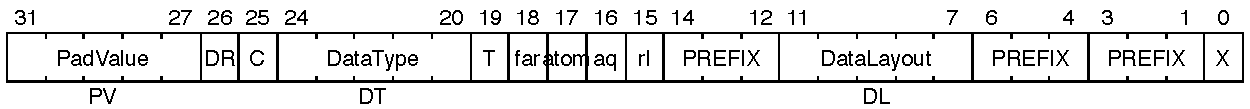
\includegraphics[width=0.95\linewidth]{figs/encoding/pto_b_attr_instruction.pdf}
\end{center}

\begin{longtable}{@{}L{0.14\linewidth}L{0.18\linewidth}R{0.08\linewidth}L{0.50\linewidth}@{}}
\toprule
Bits & Field & Width & Meaning \\
\midrule
\texttt{31:27} & \texttt{PadValue} & 5 & Pad or fill selector used by valid-region and padding profiles. \\
\texttt{26} & \texttt{DR} & 1 & Descriptor-refinement bit. Opcode profiles define whether it enables destination-role refinement. \\
\texttt{25} & \texttt{C} & 1 & Cache/control refinement bit for profiles that define it. \\
\texttt{24:20} & \texttt{DataType} & 5 & Optional format refinement. If present, it refines \texttt{B.OP.DataType}. \\
\texttt{19} & \texttt{T} & 1 & Transpose or tile-layout refinement bit, profile-defined. \\
\texttt{18} & \texttt{far} & 1 & Far-memory or far-target refinement bit, profile-defined. \\
\texttt{17} & \texttt{atom} & 1 & Atomic operation refinement bit for profiles that support atomic tile effects. \\
\texttt{16} & \texttt{aq} & 1 & Acquire ordering bit. \\
\texttt{15} & \texttt{rl} & 1 & Release ordering bit. \\
\texttt{14:12} & \texttt{Selector} & 3 & Attribute descriptor selector and subform. \\
\texttt{11:7} & \texttt{DataLayout} & 5 & Optional layout selector. See Section~\ref{sec:layout_sel}. \\
\texttt{6:1} & \texttt{Pattern} & 6 & Descriptor pattern bits for \texttt{B.ATTR}. \\
\texttt{0} & \texttt{Marker} & 1 & 32-bit descriptor marker. Fixed to 1. \\
\bottomrule
\end{longtable}

\subsection{\texttt{B.IOR} --- Scalar IO Descriptor}
\label{sec:b_ior_descriptor}
\texttt{B.IOR} imports or exports scalar values for a tile instruction bundle. Its scalar fields use the same 5-bit register IDs as scalar instructions.

\begin{center}
\captionof{figure}{Bit allocation for the \texttt{B.IOR} scalar IO descriptor.}
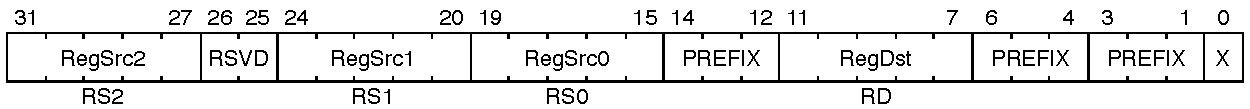
\includegraphics[width=0.95\linewidth]{figs/encoding/pto_b_ior_instruction.pdf}
\end{center}

\begin{longtable}{@{}L{0.14\linewidth}L{0.18\linewidth}R{0.08\linewidth}L{0.50\linewidth}@{}}
\toprule
Bits & Field & Width & Meaning \\
\midrule
\texttt{31:27} & \texttt{RegSrc2} & 5 & Third scalar source register \texttt{X0}--\texttt{X31}. \\
\texttt{26:25} & \texttt{RSV} & 2 & Reserved. Encoders write zero. \\
\texttt{24:20} & \texttt{RegSrc1} & 5 & Second scalar source register \texttt{X0}--\texttt{X31}. \\
\texttt{19:15} & \texttt{RegSrc0} & 5 & First scalar source register \texttt{X0}--\texttt{X31}. \\
\texttt{14:12} & \texttt{Selector} & 3 & Descriptor selector for scalar IO. \\
\texttt{11:7} & \texttt{RegDst} & 5 & Destination scalar register \texttt{X0}--\texttt{X31}. Writes to \texttt{X0} are ignored. \\
\texttt{6:1} & \texttt{Pattern} & 6 & Descriptor pattern bits. \\
\texttt{0} & \texttt{Marker} & 1 & 32-bit instruction marker. Fixed to 1. \\
\bottomrule
\end{longtable}

\subsection{\texttt{B.DIM} --- Dimension Descriptor}
\label{sec:b_dim_descriptor}
Dimension descriptors carry shape, valid-region, or loop-bound values for the selected tile opcode. \texttt{B.DIM} is always a 32-bit descriptor instruction in this revision. Smaller dimension descriptor forms are reserved and MUST NOT be emitted.

\begin{center}
\captionof{figure}{Bit allocation for the \texttt{B.DIM} dimension descriptor.}
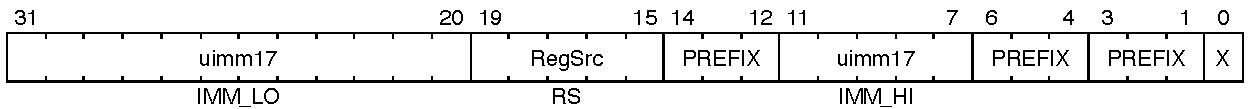
\includegraphics[width=0.95\linewidth]{figs/encoding/pto_b_dim_instruction.pdf}
\end{center}

\begin{longtable}{@{}L{0.14\linewidth}L{0.18\linewidth}R{0.08\linewidth}L{0.50\linewidth}@{}}
\toprule
Bits & Field & Width & Meaning \\
\midrule
\texttt{31:20} & \texttt{DimImmLo} & 12 & Low immediate dimension payload or profile-defined bound value. \\
\texttt{19:15} & \texttt{RegSrc} & 5 & Scalar source register \texttt{X0}--\texttt{X31} when the dimension is register-sourced. \\
\texttt{14:12} & \texttt{Selector} & 3 & Dimension selector. Values identify row, column, lane, reduction, or profile-defined bounds. \\
\texttt{11:7} & \texttt{DimImmHi} & 5 & High immediate dimension payload or profile-defined bound extension. \\
\texttt{6:1} & \texttt{Pattern} & 6 & Descriptor pattern bits for \texttt{B.DIM}. \\
\texttt{0} & \texttt{Marker} & 1 & 32-bit descriptor marker. Fixed to 1. \\
\bottomrule
\end{longtable}

\subsection{\texttt{B.IOT}/\texttt{B.IOTI} --- Tile IO Descriptor}
\label{sec:b_iot_summary}
\texttt{B.IOT}/\texttt{B.IOTI} carries tile input/output bindings for a tile instruction bundle. The descriptor has one source-list plus arrow-destination layout: \texttt{SrcTile0}/\texttt{SrcTile1} name explicit tile inputs, \texttt{S0V}/\texttt{S1V} mark absent inputs, reuse bits annotate source lifetime, and \texttt{DstTile} plus the arrow suffix names the destination kind. \texttt{B.IOTI} uses bits \texttt{11:7} as an immediate tile \texttt{SizeCode}; \texttt{B.IOT} uses the same field as a scalar \texttt{RegSrc} only when the opcode profile enables dynamic sizing.

\begin{center}
\captionof{figure}{Bit allocation for the \texttt{B.IOTI} immediate-size tile IO descriptor.}
\includegraphics[width=0.95\linewidth]{figs/encoding/pto_b_ioti_instruction.pdf}
\end{center}

\begin{longtable}{@{}L{0.14\linewidth}L{0.18\linewidth}R{0.08\linewidth}L{0.50\linewidth}@{}}
\toprule
Bits & Field & Width & Meaning \\
\midrule
\texttt{31} & \texttt{S1R} & 1 & Source 1 reuse hint. \\
\texttt{30} & \texttt{S0R} & 1 & Source 0 reuse hint. \\
\texttt{29} & \texttt{S1V} & 1 & Source 1 absent flag. \\
\texttt{28} & \texttt{S0V} & 1 & Source 0 absent flag. \\
\texttt{27:25} & \texttt{DstTile} & 3 & Destination kind for the arrow binding: tile hand or accumulator, interpreted with the printed \texttt{->...<...>} suffix. \\
\texttt{24:20} & \texttt{SrcTile1} & 5 & Descriptor-local second source selector. \\
\texttt{19:15} & \texttt{SrcTile0} & 5 & Descriptor-local first source selector. \\
\texttt{14:12} & \texttt{selector} & 3 & Tile IO selector and profile subform. The generated fixed-size tile pages use \texttt{110} for continue and \texttt{111} for the last \texttt{B.IOTI} descriptor. \\
\texttt{11:7} & \texttt{SizeCode/RegSrc} & 5 & Immediate size code for \texttt{B.IOTI}; scalar size source register for dynamic-size \texttt{B.IOT} profiles. \\
\texttt{6:1} & \texttt{Pattern} & 6 & Descriptor pattern bits. \\
\texttt{0} & \texttt{Marker} & 1 & 32-bit descriptor marker. Fixed to 1. \\
\bottomrule
\end{longtable}

\subsection{Bundled Descriptor Summary}
\begin{longtable}{@{}L{0.14\linewidth}L{0.08\linewidth}L{0.09\linewidth}L{0.09\linewidth}L{0.10\linewidth}L{0.42\linewidth}@{}}
\toprule
Mnemonic & Length & bits[3:1] & bits[6:4] & bits[14:12] & Key field ranges \\
\midrule
\texttt{B.OP} & 32-bit & 000 & 000 & 001 & \texttt{DataType}, \texttt{Mode}, \texttt{Opcode}, and descriptor kind fields \\
\texttt{B.ATTR} & 32-bit & 001 & 001 & profile & \texttt{PadValue}, \texttt{DataType}, \texttt{DataLayout}, ordering and profile refinement bits \\
\texttt{B.ARG} & 32-bit & 001 & 100 & 011 & bits[11:7] profile argument \\
\texttt{B.DIM} & 32-bit & 001 & 100 & 0/1/2 & Immediate and scalar-register dimension fields \\
\texttt{B.IOR} & 32-bit & 001 & 001 & 000 & bits[31:27] \texttt{RegSrc2}, bits[24:20] \texttt{RegSrc1}, bits[19:15] \texttt{RegSrc0}, bits[11:7] \texttt{RegDst} \\
\texttt{B.IOT} & 32-bit & 001 & 001 & 100/101 & Tile source/destination selectors plus scalar size source register for dynamic-size profiles \\
\texttt{B.IOTI} & 32-bit & 001 & 001 & 110/111 & Tile source/destination selectors plus immediate size code; \texttt{111} marks the last descriptor in a repeated tile IO group \\
\texttt{B.TEXT} & 32-bit & 001 & 000 & 000 & bits[31:7] signed PC-relative target offset \\
\texttt{B.HINT} & 32-bit & 001 & 011 & 000/001 & Prefetch, temperature, trace, or branch-likelihood hint fields \\
\bottomrule
\end{longtable}

\index{bundled descriptor encoding summary}\index{descriptor encoding table}

\clearpage
